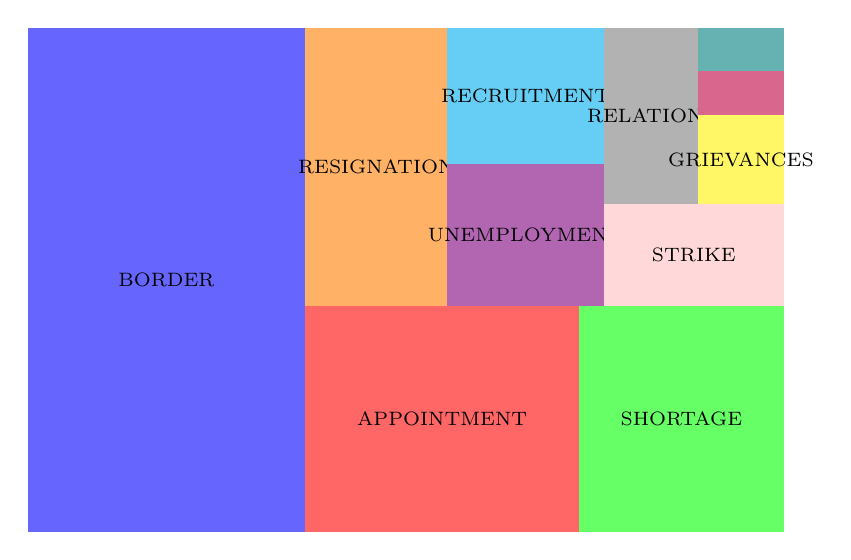
\begin{tikzpicture}[x=0.08cm,y=0.08cm]
% Auto-generated squarified treemap
% Data: 11 items, total value: 1,387,384
\fill[blue!60] (0.00,0.00) rectangle (44.06,80.00);
\node[align=center,font=\scriptsize] at (22.03,40.00) {BORDER};
\fill[red!60] (44.06,0.00) rectangle (87.54,35.85);
\node[align=center,font=\scriptsize] at (65.80,17.92) {APPOINTMENT};
\fill[green!60] (87.54,0.00) rectangle (120.00,35.85);
\node[align=center,font=\scriptsize] at (103.77,17.92) {SHORTAGE};
\fill[orange!60] (44.06,35.85) rectangle (66.60,80.00);
\node[align=center,font=\scriptsize] at (55.33,57.92) {RESIGNATION};
\fill[violet!60] (66.60,35.85) rectangle (91.51,58.36);
\node[align=center,font=\scriptsize] at (79.05,47.10) {UNEMPLOYMENT};
\fill[cyan!60] (66.60,58.36) rectangle (91.51,80.00);
\node[align=center,font=\scriptsize] at (79.05,69.18) {RECRUITMENT};
\fill[pink!60] (91.51,35.85) rectangle (120.00,51.94);
\node[align=center,font=\scriptsize] at (105.76,43.89) {STRIKE};
\fill[gray!60] (91.51,51.94) rectangle (106.48,80.00);
\node[align=center,font=\scriptsize] at (99.00,65.97) {RELATIONS};
\fill[yellow!60] (106.48,51.94) rectangle (120.00,66.15);
\node[align=center,font=\scriptsize] at (113.24,59.04) {GRIEVANCES};
\fill[purple!60] (106.48,66.15) rectangle (120.00,73.15);
\fill[teal!60] (106.48,73.15) rectangle (120.00,80.00);
\end{tikzpicture}